\documentclass[11pt,a4paper]{article}
\usepackage[utf8]{inputenc}
\usepackage[T1]{fontenc}
\usepackage[polish]{babel}
\usepackage{lmodern}
\usepackage{graphicx}
\usepackage{epstopdf}
\usepackage{anysize}
\usepackage{makeidx}
\usepackage{hyperref}



\makeatletter
\renewcommand{\maketitle}{
\begin{titlepage}
\begin{center}

\LARGE{AKADEMIA GÓRNICZO-HUTNICZA}

\vspace*{1cm}

\includegraphics[scale=1.8]{agh.eps}
\vspace*{1cm}

\LARGE{im. Stanisława Staszica w Krakowie}

\rule{\textwidth}{0.4mm}
\LARGE \textsc{\@title}
\rule{\textwidth}{0.4mm}

\vspace*{5mm}


\large
\emph{Autorzy:}\\
Bartłomiej \textsc{Bułat}\\
Tomasz \textsc{Czarnik}\\
Krzysztof \textsc{Śmiłek}\\

\vfill
\vspace*{\stretch{8}}
\rule{\textwidth}{0.4mm}

\large{Wydział Elektroniki, Automatyki, Informatyki i Elektrotechniki}\\
\large{Katedra Automatyki}\\
\large{Laboratorium Biocybernetyki}\\
\vspace*{\stretch{7}}
\@date

\end{center}

\end{titlepage}
}
\makeatother

\title{Badanie metod rozpoznawania\\twarzy na obrazach}
\date{\today}

\makeindex

\begin{document}

\maketitle

\newpage

\tableofcontents

\newpage

\section{Metody geometryczne}
W metodach tych twarz charakteryzowana jest przez zbiór wartości kątów, odległości czy też pól wyznaczonych w oparciu o charakterystyczne punkty, takie jak środki oczu, koniec nosa itd. Problemem jest tutaj precyzyjne zlokalizowanie odpowiednich fragmentów twarzy. Staje się to szczególnie trudne gdy zdjęcie poddane analizie nie jest wykonane bezpośrednio od przodu, gdyż wówczas niektóre istotne części twarzy mogą być nawet całkowicie niewidoczne. Sporządzanie opisu matematycznego poprzez wyznaczenie geometrycznych parametrów było jednym z pierwszych, najbardziej intuicyjnych pomysłów na ekstrakcję cech w rozpoznawaniu twarzy. Obecnie jednak podejście to praktycznie nie jest już rozwijane, gdyż istnieją mechanizmy wykrywające twarze szybciej oraz z większą skutecznością.

\section{Metoda analizy kolorów}
W metodzie tej na podstawie odpowiednich schematów kolorów wykrywa się wszystkie elementy na obrazie zgodne z danym schematem. Niestety metoda ta jest bardzo wrażliwa ponieważ poza twarzą wykrywa też dłonie, szyję itp. Dlatego też dodatkowo zwykle należy przeprowadzić po niej selekcję po kształcie i rozmiarze wykrytych regionów. 
\\
\\
\noindent Zalety:
\begin{itemize}
\item szybkość
\item brak ograniczeń odnośnie orientacji oraz rozmiaru twarzy
\end{itemize}

\noindent Wady:
\begin{itemize}
\item baza schematów kolorów jest ograniczona
\item duża podatność metody na natężenie jasności zdjęcia
\item obiekty o kolorze podobnym do koloru skóry są także wykrywane
\end{itemize}

\section{Metoda Sieci neuronowych}
Operację wykrywania twarzy za pomocą tego systemu można podzielić na 3 główne składowe:
\begin{enumerate}
\item Inicjalizacja (projektowanie i tworzenie sieci neuronowych)
\item Trening (wybór danych do trenowania, wybór cech, właściwe trenowanie)
\item Klasyfikacja (skanowanie obrazów w celu zlokalizowania twarzy)
\end{enumerate}

\noindent 
Do tego celu tworzone są jednokierunkowe warstwowe sieci neuronowe, które są trenowane przy użyciu metody wstecznej propagacji. Dane treningowe zawierają obrazy z twarzami lub bez. Przepuszczając przez sieć wybrany obraz, równocześnie na wyjściu z sieci ustalamy ostateczny wynik (1 – twarz, -1 – obraz bez twarzy).  Dzięki wspomnianej wcześniej metody wstecznej propagacji, na podstawie wyjścia z całej sieci, komórki wewnętrzne są w stanie same kalibrować swoje wartości tak, aby sprostać wymogom całej sieci.\\
Poddając dany obraz badaniu na obecność twarzy, jest on skalowany i dzielony na okna, które są indywidualnie przepuszczane przez sieć. Okna, które zawierają twarze są otaczane obwiednią, następnie wszystkie okna są łączone ponownie w całość i następuje skalowanie obrazu do pierwotnego rozmiaru. Dzięki temu na obrazie końcowym możemy ujrzeć przeskalowane prostokąty, które wskazują, w którym konkretnie miejscu znaleziono twarze.

\vspace*{1cm}
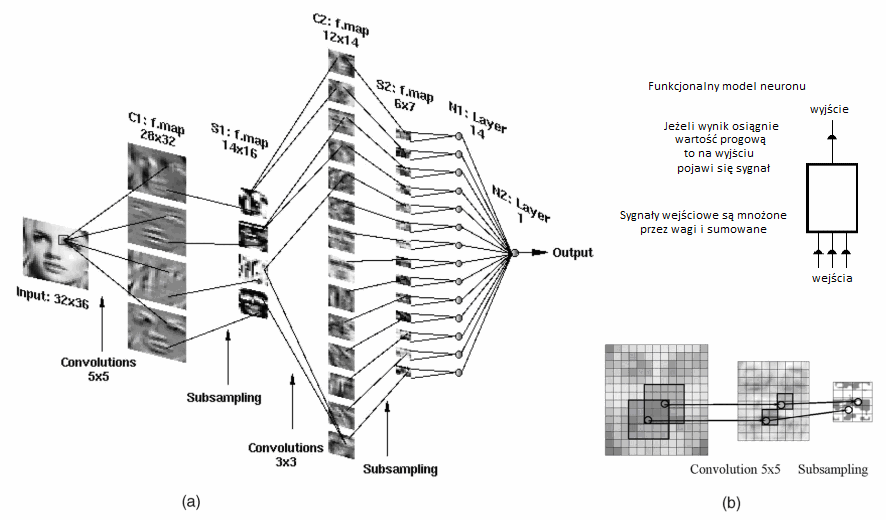
\includegraphics[scale=0.65]{cnn.png}
\vspace*{1cm}

\noindent 
Zalety:
\begin{itemize}
\item  Bardzo dobre rozpoznawanie wzorców
\item  Praca z zaszumianymi i niepełnymi danymi
\item  Możliwość pracy równoległa z wielu wejść
\item  Rozwiązanie problemu bez jego dogłębnej analizy
\item  Duża tolerancja na błędy
\end{itemize}

\noindent 
Wady:
\begin{itemize}
\item  Długi czas uczenia 
\item  Sukces uczenia nie jest gwarantowany 
\item  Problemy z wyborem danych do treningu sieci 
\end{itemize}

\end{document}
